\documentclass[licencjacka]{pracamgr_Kogni}
\usepackage{setspace}
\usepackage{natbib}
\usepackage{xcolor}
\usepackage{graphicx}
\usepackage{hyperref} 
 \hypersetup{ 
     colorlinks=true,
     linkcolor=black,
     citecolor=black,
     urlcolor=darkgray,
     }
\onehalfspacing
\autor{Kamil Tomaszek}{432044}
\title{Minimalizacja długości zależności w~strukturach współrzędnie złożonych: badanie korpusowe na~podstawie Polish Dependency Bank}
\kierunek{kognitywistyka}
\opiekun{\\ 
\bfseries prof. dr hab. Adama Przepiórkowskiego\\
Uniwersytet Warszawski}
\date{czerwiec 2023}
\keywords{koordynacja, minimalizacja długości zależności, Polish Dependency Bank, drzewo zależnościowe, korpus języka polskiego}

\begin{document}

\maketitle

\tytulang{Dependency Length Minimisation in coordinate structures: A corpus study based on \\ Polish Dependency Bank}

\begin{abstract}
Praca licencjacka na temat "Minimalizacja długości zależności w strukturach współrzędnie złożonych: badanie korpusowe na podstawie Polish Dependency Bank"  jest poświęcona zjawisku minimalizacji długości zależności (DLM) w koordynacji w języku polskim. Celem pracy jest sprawdzenie hipotez na ten temat oraz przedstawienie dodatkowych analiz. Ma ona charakter empiryczny i opiera się na danych pochodzących z Polish Dependency Bank (PDB). Praca składa się z sześciu rozdziałów. W pierwszym rozdziale przedstawiłem motywację, cel i zakres pracy oraz jej strukturę. W drugim rozdziale omówiłem teoretyczne podstawy pracy, tj. reprezentacje koordynacji w języku polskim, teorię zależności składniowej i DLM w koordynacji. W trzecim rozdziale opisałem źródło danych i narzędzia do analizy, tj. PDB i preprocessing
danych za pomocą algorytmu napisanego w Pythonie. W czwartym rozdziale zaprezentowałem wyniki analizy statystycznej wykonanej w R oraz testowanie hipotez za pomocą m. in. testu chi-kwadrat. W piątym rozdziale dokonałem dyskusji wyników, interpretacji ich znaczenia i porównania z literaturą naukową. W szóstym rozdziale podsumowałem pracę i wnioski oraz zaproponowałem perspektywy dalszych badań.
\end{abstract}

\thispagestyle{empty}
\setcounter{page}{3}
\tableofcontents 

\chapter{Wstęp}
W tym rozdziale przedstawiam motywację i cel pracy licencjackiej na temat "Minimalizacja długości zależności w strukturach współrzędnie złożonych: badanie korpusowe na podstawie Polish Dependency Bank", a także omawiam jej zakres oraz strukturę.

\section{Motywacja i cel pracy}

Praca ta ma na celu analizę zjawiska minimalizacji długości zależności – DLM (z ang. Dependency Length Minimisation), czyli tendencji do umieszczania elementów współrzędnych o różnych długościach w sposób, by zmniejszyć odległość zarówno między nimi samymi, jak i między nimi a innymi elementami zdania, w koordynacjach w języku polskim. Koordynacja to zjawisko, gdy wiele części zdania ma jeden nadrzędnik i każda z nich się z nim koordynuje. Zjawisko to jest istotne dla teorii składniowej i reprezentacji językowych, ponieważ dotyczy zarówno formy jak i znaczenia zdań. W pracy tej sprawdzono dwie hipotezy dotyczące długości członów w koordynacjach w języku polskim: 1. że dłuższy człon koordynacji jest częściej ze strony prawej i 2. że dłuższy człon koordynacji jest częściej dalej od jej nadrzędnika.
\\

(0) \textit{Widziałem} Asię \textbf{i} jej śmiesznego, młodszego brata. \\
\\
Długości członów mierzono na cztery różne sposoby, licząc znaki, sylaby, słowa oraz tokeny. W przykładzie (0) odpowiednie wartości wynosiłyby [4~vs~31, 2~vs~9, 1~vs~4, 1~vs~5]. Szybko pokazano, że jedna z hipotez zachodzi w większości przypadków, więc następnie omówiono wpływ obecności i pozycji nadrzędnika oraz długości różnicy między analizowanymi członami na proporcje danych, w których hipoteza ta jest prawdziwa. Praca ta ma charakter empiryczny, opiera się na danych pochodzących z Polish Dependency Bank (PDB), czyli korpusu języka polskiego zawierającego ponad 22 tysiące drzew zależnościowych oraz na podobnej pracy badającej te same zależności, ale dla języka angielskiego \citep{AnonimoweNieopublikowane}.

\section{Zakres i struktura pracy}
Praca składa się z sześciu rozdziałów. W rozdziale drugim omówiono teoretyczne podstawy pracy, tj. przedstawiono czym są koordynacje -- na przykładzie języka polskiego, zaprezentowano zarys teorii zależności składniowej, opisano minimalizację teorii zależności oraz wskazano różne reprezentacje zależnościowe wraz z ich przewidywaniami. W rozdziale trzecim opisano źródło danych, czyli Polish Dependency Bank, jak i ich preprocessing -- działanie algorytmu, napisanego w języku Python, wybierającego koordynacje oraz informacje o nich z PDB, a także pokazano format danych po preprocessingu w pliku z rozszerzeniem ".csv". W rozdziale czwartym zaprezentowano hipotezy badawcze, ich testowanie wraz z analizami statystycznymi w języku R (m. in. test Wilcoxona, testy chi-kwadrat oraz ogólne modele liniowe [GLM – z ang. Generalised Linear Models]). W rozdziale piątym omówiono wyniki badań i ich interpretację w kontekście istniejącej wcześniej literatury naukowej. W rozdziale szóstym podsumowano pracę, wyciągnięto z niej wnioski oraz zaproponowano perspektywy dalszych badań. 

\chapter{Teoretyczne podstawy minimalizacji długości zależności w strukturach współrzędnie złożonych}
W tym rozdziale omawiam teoretyczne podstawy pracy, tj. opisuję czym są koordynacje, przedstawiam zarys teorii zależności składniowej, prezentuję minimalizację teorii zależności oraz wskazuję różne reprezentacje zależnościowe wraz z ich przewidywaniami.

\section{Koordynacja w języku polskim}
Zacznę od przedstawienia pojęcia koordynacji. Koordynacja to zjawisko w językach naturalnych, które zachodzi w struktruach złożonych -- zarówno współrzędnie, jak i podrzędnie. Polega na zestawieniu dwóch lub więcej elementów o tej samej funkcji składniowej za pomocą spójników lub interpunkcji i tym samym złączenie ich w jeden, większy element, zachowujący te same funkcje składniowe. Jest ono jednym z podstawowych sposobów łączenia słów, czy zdań. Elementami koordynacji mogą być zarówno pojedyncze słowa (1a, 1b),  wyrażenia (1c), jak i całe zdania (1d):
\\

(1)

a. Ania \textbf{i} Julia \textit{idą} na spacer.

b. Ania \textbf{i} Julia.

c. Wesoła Marysia \textbf{oraz} smutny Janek \textit{wybrali się} do parku.

d. \textit{Kuba} zjadł obiad \textbf{a} następnie poszedł spać.
\\
\\
Człony koordynacji nazywamy koordynantami, to co je łączy -- spójnikiem koordynacji (w przykładach w tej pracy jest on ilustrowany pogrubionym tekstem), a wyraz nadrzędny względem obu członów -- głową koordynacji (w przykładach ilustrowany kursywą). Jak widać w (1b) nie zawsze istnieje głowa koordynacji.
W podanych wyżej przykładach koordynantami są: (1a, 1b) Ania, Julia; (1c) Wesoła Marysia, smutny Janek; (1d) zjadł obiad, poszedł spać.

Ze względów semantycznych zwykle wyróżnia się cztery rodzaje koordynacji: koordynacje koniunkcyjne (2a), koordynacje dysjunkcyjne (2b), koordynacje adwersatywne (2c) oraz koordynacje kauzalne (2d) \citep{Haspelmath2007}. Każde z nich używają różnych zestawów spójników, które łączą koordynanty. W koordynacjach koniunkcyjnych koordynanty łączą m. in. spójniki [i, oraz, ani, tudzież, również], a w koordynacjach dysjunkcyjnych -- [albo, bądź, lub, czy], lecz w obu tych kategoriach wykorzystywana jest także interpunkcja. W koordynacjach adwersatywnych używamy m. in. spójników [ale, lecz, zaś, natomiast, jednak], a w koordynacjach kauzalnych -- [bo, ponieważ, dlatego że]. W tej pracy skupię się na pierwszych trzech rodzajach koordynacji, jako że to one występują w strukturach współrzędnie złożonych.
\\

(2)

a. Marta \textit{zjadła} jabłko \textbf{i} gruszkę.

b. Ona miała szesnaście \textbf{lub} siedemnaście \textit{lat}.

c. \textit{Byli} ładni, \textbf{ale} głupi.

d. Nie zrobiłem pracy domowej, \textbf{bo} nie chciałem.

\section{Zarys teorii zależności składniowej}
Teoria zależności składniowej jest jednym z głównych podejść do analizy struktury zdania w lingwistyce. Teoria ta zakłada, że każde zdanie składa się z korzenia (root) i zależnych od niego elementów, które są połączone za pomocą krawędzi drzewa składniowego.\\
Teoria ta opiera się na kilku podstawowych założeniach \citep{Liu2008}:\\
- Struktura zdania wynika z zależności pomiędzy słowami, a nie z ich kolejności. W tym podejściu, zdanie jest analizowane jako złożenie zależności między jego elementami, a nie jako sekwencja słów, jak w tradycyjnym podejściu gramatycznym.\\
- Każda relacja między elementami jest relacją między dokładnie dwoma elementami\\
- Zazwyczaj relacje zależności są asymetryczne, jednokierunkowe, gdzie jeden z elementów jest korzeniem (lokalnym), a drugi elementem od niego zależnym.\\
- Korzeń zdania jest najważniejszym elementem, który określa jego znaczenie i funkcję komunikacyjną. \\
- Zależności są oznaczane etykietami, które określają funkcje syntaktyczne elementów zależnych.\\
- Zmiana kolejności słów w zdaniu nie wpływa na jego strukturę zależnościową, a jedynie na jego znaczenie pragmatyczne lub stylistyczne.
\\

\begin{figure}
    \hspace{0.7cm}(3) Drzewo składniowe dla przykładowego zdania z PDB:

    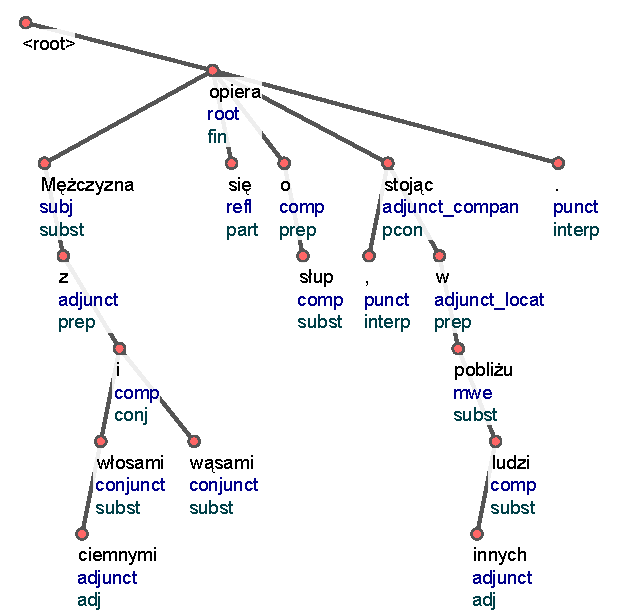
\includegraphics{drzewko.pdf}

    Mężczyzna z ciemnymi włosami i wąsami opiera się o słup, stojąc w pobliżu innych ludzi.
\end{figure}

Powyższe drzewo zależnościowe należy odczytywać w konkretny sposób. Elementy, które są niżej są zależne od elementów znajdujących się wyżej, z którymi są połączone. Korzeń znajduje się na samej górze. Tekst pod etykietami słów oznacza: niebieski -- funkcje, które pełnią w zdaniu oraz zielony -- tzw. \textit{tagi} danych wyrazów. W tym przypadku, słowo \textbf{opiera} jest korzeniem zdania.

Teoria zależności składniowej ma długą i bogatą historię, która sięga aż starożytności. Pierwsze ślady tego podejścia można znaleźć w gramatyce sanskrytu Pāṇiniego, czy w pracach wczesnych arabskich gramatyków \citep{Kruijff2002}, a także w niektórych teoriach gramatycznych średniowiecza \citep{Covington1984}. W XX wieku teoria ta mocno rozwinęła się zwłaszcza w lingwistyce klasycznej i słowiańskiej \citep{Melcuk1988}. \citet{Tesniere1959} podjął próvę stworzenia kompleksowej teorii gramatyki, w której to wszystko byłoby oparte na zależnościach. Przedstawił on jej potencjał do uchwycenia podobieństw, jak i różnic między językami.

Teoria zależności składniowej jest popularnym podejściem w dziedzinie przetwarzania języka naturalnego, ponieważ umożliwia łatwe i precyzyjne analizowanie struktury zdania i wyrażanie jej za pomocą drzew zależnościowych. Ma ona wiele zastosowań, np. w dziedzinach takich jak tłumaczenie maszynowe czy analiza sentymentu, ponieważ ułatwia przetwarzanie i rozumienie znaczenia zdań. W ostatnich latach powstały projekty takie jak Universal Dependencies (\url{https://universaldependencies.org/}), które mają na celu zunifikowanie reprezentacji lingwistycznych (w tym wypadku: morfosyntaktycznej) dla różnych języków. Dla języka polskiego stworzono już kilka wersji tego korpusu \citep{Przepiorkowski2020} oraz cały czas się on rozwija na kolejne języki.

\section{Minimalizacja długości zależności}
Minimalizacja długości zależności (DLM) to zasada, według której języki naturalne dążą do zmniejszania odległości między słowami zależnymi syntaktycznie. Zasada ta jest odnotowywana w lingwistyce już od długiego czasu i pozwala nam na bardziej efektywne analizowanie i generowanie języka naturalnego. W ciągu ostatnich 20 lat hipoteza o nacisku na DLM została wykorzystana do wyjaśnienia wielu z najbardziej uniwersalnych właściwości języków \citep{FutrellEtAl2015}.
Jak twierdzą \citet{Hawkins1994} i \citet{FutrellEtAl2020}, rozróżniamy jej występowanie na poziom gramatyczny, jak i codzienne użycie języka. \citet{Liu2008} twierdzi, że długości zależności mogłyby być wskaźnikiem trudności danego języka, sugerując przy tym pewną uniwersalność stosowania DLM w celu łatwiejszego zrozumienia mowy i pisma.

Według DLM, jeśli oba ustawienia członów koordynacji binarnych (jeden człon raz z lewej strony, raz z prawej) są gramatycznie poprawne, to bliżej głowy znajdzie się krótszy człon. W przykładach (4a, 4b) oba ustawienia wydają się brzmieć naturalnie, jednak gdy wydłużymy jeden z członów -- w (4c, 4d), zauważymy, że bardziej naturalne będzie ustawienie krótszego członu z lewej strony.
\\

(4)

a. \textit{Nie ma} Kamila \textbf{i} Julii.

b. \textit{Nie ma} Julii \textbf{i} Kamila.

c. \textit{Nie ma} Kamila \textbf{i} wiecznie spóźnionej Julii.

d. \textit{Nie ma} wiecznie spóźnionej Julii \textbf{i} Kamila.
\\
\\
\citet{Hawkins1994} argumentuje, że DLM występuje w gramatyce, ale niekoniecznie w użyciu codziennym. Jako powód wskazuje, że w języku angielskim kolejność V-NP-PP (V - czasownik [z ang. verb], NP - fraza rzeczownikowa [z ang. nominal phrase], PP - fraza przyimkowa [z ang. prepositional phrase]) występuje częsciej niż V-PP-NP nie tylko gdy NP jest krótsze od PP, ale i wtedy gdy są podobnej długości. Używa on tego przykładu, ponieważ jest on jednym z tych, które uważa się za ilustrujące występowanie DLM (jako że NP są zazwyczaj krótsze niż PP). Słowa Hawkinsa dla języka angielskiego ilustrują przykłady (5a, 5b), w których kolejność V-NP-PP jest bardziej naturalna niż V-PP-NP), mimo że obie frazy są podobnej długości. Zdanie (5c) również brzmi jednak naturalnie, co wskazuje na pewien wpływ dodatkowego czynnika --  długości różnicy obu członów koordynacji na to, czy DLM będzie w danym przypadku zachowana.
\\

(5)

a. I gave <a book> <to John>. [Dałem <książkę> <Johnowi>.]

b. I gave <to John> <a book>. [Dałem <Johnowi> <książkę>.]

c. I gave <to John> <the most interesting book I've read in years>. [Dałem <Johnowi> <najbardziej interesującą książkę, jaką przeczytałem od lat>.]\\
za: \citet{AnonimoweNieopublikowane}
\\
\\
Jednym ze sposobów na badanie DLM jest tworzenie sztucznych języków losowych (w których kolejność słów, czy relacje zależności są losowo dobierane) oraz porównywanie długości zależności w tych językach z długościami zależności w językach naturalnych. Badania wykazały, że języki naturalne mają istotnie krótsze długości zależności niż sztucznie wygenerowane wartości dla przykładowych losowych języków \citep{FutrellEtAl2015}, co sugeruje, że istnieje uniwersalna tendencja u ludzi do wykorzystywania DLM.

DLM jest również powiązana z innymi właściwościami języków naturalnych, takimi jak projektywność i finalność głowy. Projektywność oznacza brak lub rzadkość przecinających się zależności, które wydłużają długość zależności. Finalność głowy oznacza kierunek występowania nadrzędnika frazy względem jej dopełnienia. Badania wykazały, że istnieje związek między finalnością głowy a długością zależności, przy czym języki o finalności głowy na końcu zdania mają krótszą długość zależności niż języki o finalności głowy na początku zdania \citep{FutrellEtAl2015}.

DLM nie jest jednak jedynym czynnikiem kształtującym strukturę syntaktyczną języków naturalnych. Istnieją również inne ograniczenia i preferencje, takie jak harmonia języka \citep{Jing2022}, czy preferencje semantyczne, które mogą wpływać na kolejność słów i długość zależności. Niektóre z tych czynników mogą być sprzeczne lub komplementarne względem DLM. Dlatego DLM należy rozumieć jako jeden z wielu czynników wpływających na organizację języka naturalnego.

\section{Różne reprezentacje koordynacji}
Tekst sekcji

\chapter{Polish Dependency Bank -- źródło danych i narzędzia do analizy}
Tekst rozdziału
\section{Krótki opis Polish Dependency Bank}
Tekst sekcji
\section{Preprocessing danych}
Tekst sekcji
\section{Dane po preprocessingu}
Tekst sekcji

\chapter{Analiza statystyczna}
Tekst rozdziału
\section{Hipoteza, metody}
Tekst sekcji
\section{Przedstawienie wyników analizy statystycznej w R}
Tekst sekcji
\section{Testowanie hipotez}
Tekst sekcji

\chapter{Dyskusja wyników}
Tekst rozdziału
\section{Podsumowanie wyników badań}
Tekst sekcji
\section{Interpretacja wyników}
Tekst sekcji
\section{Przegląd literatury}
Tekst sekcji

\chapter{Zakończenie}
Tekst rozdziału
\section{Podsumowanie pracy i wnioski}
Tekst sekcji
\section{Perspektywy dalszych badań}
Tekst sekcji

\begin{thebibliography}{99}
\addcontentsline{toc}{chapter}{Bibliografia}

\bibitem [Anonimowe Zgłoszenie na ACL(nieopublikowane)]{AnonimoweNieopublikowane}
Anonimowe Zgłoszenie na ACL 2023 (nieopublikowane). Conjunct Lengths in English, Dependency Length Minimization, and Dependency Structure of Coordination

\bibitem[Covington(1984)]{Covington1984}
Covington, M.A. (1984). \textit{Syntactic Theory in the High Middle Ages: Modistic Models of Sentence Structure}
(Cambridge Studies in Linguistics). Cambridge: Cambridge University Press. Za: de Marneffe, M.-C. \& Nivre, J. (2019). Dependency Grammar. \textit{Annual Review of Linguistics} 5, 197-218. \url{https://doi.org/10.1146/annurev-linguistics-011718-011842}

\bibitem [Futrell et al.(2015)]{FutrellEtAl2015}
Futrell, R., Mahowald, K., \& Gibson, E. (2015). Large-scale evidence of dependency length minimization in 37 languages. \textit{Proceedings of the National Academy of Sciences} 112(33), 10336–10341. \url{https://doi.org/10.1073/pnas.1502134112}

\bibitem [Futrell et al.(2020)]{FutrellEtAl2020}
Futrell, R., Levy R. P., \& Gibson, E. (2020). Dependency locality as an explanatory principle for word order. \textit{Language} 96(2), 371–412. Za: Anonimowe Zgłoszenie na ACL 2023 (nieopublikowane). Conjunct Lengths in English, Dependency Length Minimization, and Dependency Structure of Coordination

\bibitem [Haspelmath(2007)]{Haspelmath2007}
Haspelmath, M. (2007). Coordination. In T. Shopen (Ed.), \textit{Language typology and syntactic description, Volume II: Complex constructions} (pp. 1-51). Cambridge University Press.

\bibitem [Hawkins(1994)]{Hawkins1994}
Hawkins, J. A. (1994). A Performance Theory of Order and Constituency. \textit{Cambridge University Press}. Za: Anonimowe Zgłoszenie na ACL 2023 (nieopublikowane). Conjunct Lengths in English, Dependency Length Minimization, and Dependency Structure of Coordination

\bibitem [Jing et al.(2022)]{Jing2022}
Jing, Y., Blasi, D., \& Bickel, B. (2022). Dependency Length Minimization and Its Limits: A Possible Role for a Probabilistic Version of the Final-Over-Final Condition. \textit{Language} 98(3). \url{https://doi.org/10.1353/lan.2022.0013}. 

\bibitem [Kruijff(2002)]{Kruijff2002}
Kruijff, G.-J. M. (2002). Formal and computational aspects of dependency grammar: History and development of dg. \textit{Technical report}, ESSLI2002. Za: Pedersen, M., Eades, D. Amin, S. K. \& Prakash, L. (2004). Relative Clauses in Hindi and Arabic: A Paninian Dependency Grammar Analysis. In \textit{Proceedings of the Workshop on Recent Advances in Dependency Grammar} (pp. 9-16). Geneva, COLING

\bibitem [Liu(2008)]{Liu2008}
Liu, H. (2008). Dependency distance as a metric of language comprehension difficulty. \textit{Journal of Cognitive Science} 9(2), 159–191. \url{https://doi.org/10.17791/jcs.2008.9.2.159}

\bibitem [Mel'čuk(1988)]{Melcuk1988}
Mel'čuk, I.A. (1988). \textit{Dependency syntax: theory and practice.} SUNY press. Za: de Marneffe, M.-C. \& Nivre, J. (2019). Dependency Grammar. \textit{Annual Review of Linguistics} 5, 197-218. \url{https://doi.org/10.1146/annurev-linguistics-011718-011842}

\bibitem [Przepiórkowski \& Patejuk(2020)]{Przepiorkowski2020}
Przepiórkowski, A., Patejuk, A. (2020). From Lexical Functional Grammar to enhanced Universal Dependencies. \textit{Lang Resources \& Evaluation} 54, 185–221. \url{https://doi.org/10.1007/s10579-018-9433-z}

\bibitem [Tesnière(1959)]{Tesniere1959}
Tesnière, L. (1959). \textit{Éléments de syntaxe structurale. Préf. de Jean Fourquet.} C. Klincksieck. Za: de Marneffe, M.-C. \& Nivre, J. (2019). Dependency Grammar. \textit{Annual Review of Linguistics} 5, 197-218. \url{https://doi.org/10.1146/annurev-linguistics-011718-011842}

\end{thebibliography}


\chapter*{Załączniki}
\addcontentsline{toc}{chapter}{Załączniki}
\end{document}
